\documentclass[a4paper,landscape,8pt]{extarticle}

\usepackage[a4paper,margin=0.7cm]{geometry}

\usepackage{fancyhdr}
\pagestyle{fancy}
\fancyfoot[R]{\vspace{-35pt}\Huge\thepage}

\usepackage{multicol}
\setlength\columnsep{20pt}
\setlength{\columnseprule}{0.1pt} 

\setlength\parindent{0pt}

\usepackage[ngerman]{babel} % Silbentrennung
\usepackage[utf8]{inputenc} % Umlaute
\usepackage{microtype}

\usepackage{hyperref}

\usepackage{float}
\usepackage{graphicx}
\usepackage{wrapfig}

\usepackage{comment}

\usepackage{amsmath}
\usepackage{amssymb}

\usepackage{cancel}

\usepackage[table, dvipsnames]{xcolor}


\usepackage{booktabs}

\newenvironment{rcases}
  {\left.\begin{aligned}}
  {\end{aligned}\right\rbrace}
  
\usepackage{enumitem}
\setlist{noitemsep,topsep=3pt,parsep=3pt,partopsep=3pt,leftmargin=18pt}
\renewcommand\labelitemi{{\boldmath$\cdot$}}
\newcommand{\listarrow}{
\smash{\scalebox{1.5}[1.75]{\rotatebox[origin=c]{180}{$\Lsh$}}}
}

\usepackage{xifthen}
\newcommand{\emptyarg}[1][]{\ifthenelse{\isempty{#1}}{}{\ (#1)}}

% % % % %
% Structural
% % % % %

\newcommand{\Def}[1][]{\colorbox{defcolor}{\color{titlecolor}{\textbf{Def.\emptyarg[#1]}}}\kern+0.3ex}

\newcommand{\Theorem}[1][]{\colorbox{thmcolor}{\color{titlecolor}{\textbf{Thm.\emptyarg[#1]}}}\kern+0.3ex}

\newcommand{\Lemma}[1][]{\colorbox{thmcolor}{\color{titlecolor}{\textbf{Lem.\emptyarg[#1]}}}\kern+0.3ex}

\newcommand{\Trick}[1][]{\colorbox{trkcolor}{\color{titlecolor}{\textbf{Trick:\emptyarg[#1]}}}\kern+0.3ex}

\newcommand{\Recipe}[1][]{\colorbox{trkcolor}{\color{titlecolor}{\textbf{Recipe:\emptyarg[#1]}}}\kern+0.3ex}

\newcommand{\Method}[1][]{\colorbox{trkcolor}{\color{titlecolor}{\textbf{Method:\emptyarg[#1]}}}\kern+0.3ex}

\newcommand{\Procedure}[1][]{\colorbox{trkcolor}{\color{titlecolor}{\textbf{Procedure:\emptyarg[#1]}}}\kern+0.3ex}

\newcommand{\Bsp}[1][]{\colorbox{bspcolor}{\color{titlecolor}{\textbf{Bsp.\emptyarg[#1]}}}\kern+0.3ex}

\newcommand{\Beweis}[1][]{\colorbox{bewcolor}{\color{titlecolor}{\textbf{Proof:\emptyarg[#1]}}}\kern+0.3ex}

\newcommand{\Proof}[1][]{\colorbox{bewcolor}{\color{titlecolor}{\textbf{Proof:\emptyarg[#1]}}}\kern+0.3ex}

% % % % %
% In Text
% % % % %

\newcommand{\Bem}{\textbf{Bem: }}
\newcommand{\Warning}{\textbf{Warning: }}
\newcommand{\Wichtig}{\textbf{Wichtig: }}

% % % % %
% Colors
% % % % %

\definecolor{defcolor}{rgb}{0.75, 1, 0.75}
\definecolor{thmcolor}{rgb}{1, 0.75, 0.75}
\definecolor{bewcolor}{rgb}{1, 0.7, 0}
\definecolor{trkcolor}{rgb}{0.7, 0.95, 1}
\definecolor{bspcolor}{rgb}{1, 0.95, 0.43}
\definecolor{titlecolor}{rgb}{0,0,0}

\newcommand{\tcp}[1]{\textcolor{Orchid}{#1}}
\newcommand{\tcg}[1]{\textcolor{ForestGreen}{#1}}

% % % % %
% Math
% % % % %

\DeclareMathOperator{\DFT}{DFT}
\DeclareMathOperator{\FFT}{FFT}

\DeclareMathOperator{\arcsinh}{arcsinh}
\DeclareMathOperator{\arccosh}{arccosh}
\DeclareMathOperator{\arctanh}{arctanh}
\DeclareMathOperator{\arc}{arc}


\renewcommand\div{\operatorname{div}}
\DeclareMathOperator{\rot}{rot}
\newcommand{\laplace}{\Delta}

\DeclareMathOperator{\cis}{cis}

\DeclareMathOperator{\grad}{grad}
\DeclareMathOperator{\Hess}{Hess}


\renewcommand\Re{\operatorname{Re}}
\renewcommand\Im{\operatorname{Im}}

\newcommand{\abs}[1]{\left\lvert #1 \right\rvert}
\newcommand{\norm}[1]{\left\lVert #1 \right\rVert}
\newcommand{\scprod}[1]{\left\langle #1 \right\rangle}
\newcommand{\ceil}[1]{\left\lceil #1 \right\rceil}
\newcommand{\floor}[1]{\left\lfloor #1 \right\rfloor}

\newcommand{\diag}{\operatorname{diag}}

\newcommand{\hl}[1]{\colorbox{black!7}{$#1$}}

% MATRICES (LATIN)
\newcommand{\mat}[1]{\mathbf{#1}}
\renewcommand{\vec}[1]{\mathbf{#1}}
\newcommand*{\Hm}{\mathsf{H}}
\newcommand*{\T}{\mathsf{T}}

\newcommand{\MA}{\mat{A}}
\newcommand{\MB}{\mat{B}}
\newcommand{\MC}{\mat{C}}
\newcommand{\MD}{\mat{D}}
\newcommand{\ME}{\mat{E}}
\newcommand{\MF}{\mat{F}}
\newcommand{\MG}{\mat{G}}
\newcommand{\MH}{\mat{H}}
\newcommand{\MI}{\mat{I}}
\newcommand{\MJ}{\mat{J}}
\newcommand{\MK}{\mat{K}}
\newcommand{\ML}{\mat{L}}
\newcommand{\MM}{\mat{M}}
\newcommand{\MN}{\mat{N}}
\newcommand{\MO}{\mat{0}}
\newcommand{\MP}{\mat{P}}
\newcommand{\MQ}{\mat{Q}}
\newcommand{\MR}{\mat{R}}
\newcommand{\MS}{\mat{S}}
\newcommand{\MT}{\mat{T}}
\newcommand{\MU}{\mat{U}}
\newcommand{\MV}{\mat{V}}
\newcommand{\MW}{\mat{W}}
\newcommand{\MX}{\mat{X}}
\newcommand{\MY}{\mat{Y}}
\newcommand{\MZ}{\mat{Z}}

% MATRICES (GREEK)
\newcommand{\MGamma}{\mat{\Gamma}}
\newcommand{\MDelta}{\mat{\Delta}}
\newcommand{\MTheta}{\mat{\Theta}}
\newcommand{\MLambda}{\mat{\Lambda}}
\newcommand{\MXi}{\mat{\Xi}}
\newcommand{\MPi}{\mat{\Pi}}
\newcommand{\MSigma}{\mat{\Sigma}}
\newcommand{\MUpsilon}{\mat{\Upsilon}}
\newcommand{\MPhi}{\mat{\Phi}}
\newcommand{\MPsi}{\mat{\Psi}}
\newcommand{\MOmega}{\mat{\Omega}}

% VECTORS (LATIN)
\newcommand{\va}{\vec{a}}
\newcommand{\vb}{\vec{b}}
\newcommand{\vc}{\vec{c}}
\newcommand{\vd}{\vec{d}}
\newcommand{\ve}{\vec{e}}
\newcommand{\vf}{\vec{f}}
\newcommand{\vg}{\vec{g}}
\newcommand{\vh}{\vec{h}}
\newcommand{\vi}{\vec{i}}
\newcommand{\vj}{\vec{j}}
\newcommand{\vk}{\vec{k}}
\newcommand{\vl}{\vec{l}}
\newcommand{\vm}{\vec{m}}
\newcommand{\vn}{\vec{n}}
\newcommand{\vo}{\vec{o}}
\newcommand{\vp}{\vec{p}}
\newcommand{\vq}{\vec{q}}
\newcommand{\vr}{\vec{r}}
\newcommand{\vs}{\vec{s}}
\newcommand{\vt}{\vec{t}}
\newcommand{\vu}{\vec{u}}
\newcommand{\vv}{\vec{v}}
\newcommand{\vw}{\vec{w}}
\newcommand{\vx}{\vec{x}}
\newcommand{\vy}{\vec{y}}

% BRACES
\newcommand{\set}[1]{\left\{ #1 \right\}}
\newcommand{\dset}[2]{\left\{ #1 \ \middle| \ #2 \right\}}
\newcommand{\alg}[1]{\left\langle #1 \right\rangle}
\newcommand{\card}[1]{\left\lvert #1 \right\rvert}
\newcommand{\length}[1]{\left\lvert #1 \right\rvert}
\newcommand{\linsys}[2]{\left[\ #1 \ \middle| \ #2 \ \right]}

% NUMBER SYSTEMS
\newcommand{\E}{\mathbb{E}}
\newcommand{\bbH}{\mathbb{H}}
\newcommand{\K}{\mathbb{K}}
\newcommand{\F}{\mathbb{F}}
\newcommand{\N}{\mathbb{N}}
\newcommand{\Z}{\mathbb{Z}}
\newcommand{\Q}{\mathbb{Q}}
\newcommand{\R}{\mathbb{R}}
\newcommand{\M}{\mathbb{M}}
\newcommand{\C}{\mathbb{C}}

% CALLICGRAPHIC SHORTCUTS
\newcommand{\cA}{\mathcal{A}}
\newcommand{\cB}{\mathcal{B}}
\newcommand{\cC}{\mathcal{C}}
\newcommand{\cD}{\mathcal{D}}
\newcommand{\cE}{\mathcal{E}}
\newcommand{\cF}{\mathcal{F}}
\newcommand{\cG}{\mathcal{G}}
\newcommand{\cH}{\mathcal{H}}
\newcommand{\cI}{\mathcal{I}}
\newcommand{\cJ}{\mathcal{J}}
\newcommand{\cK}{\mathcal{K}}
\newcommand{\cL}{\mathcal{L}}
\newcommand{\cM}{\mathcal{M}}
\newcommand{\cN}{\mathcal{N}}
\newcommand{\cO}{\mathcal{O}}
\newcommand{\cP}{\mathcal{P}}
\newcommand{\cQ}{\mathcal{Q}}
\newcommand{\cR}{\mathcal{R}}
\newcommand{\cS}{\mathcal{S}}
\newcommand{\cT}{\mathcal{T}}
\newcommand{\cU}{\mathcal{U}}
\newcommand{\cV}{\mathcal{V}}
\newcommand{\cW}{\mathcal{W}}
\newcommand{\cX}{\mathcal{X}}
\newcommand{\cY}{\mathcal{Y}}
\newcommand{\cZ}{\mathcal{Z}}

% ASYMPTOTIC NOTATIONS
\newcommand{\BigO}{\mathcal{O}}

% Operators
\DeclareMathOperator{\rank}{rank}
\DeclareMathOperator*{\argmin}{arg\,min}
\DeclareMathOperator*{\argmax}{arg\,max}

% % % % %
% Layout
% % % % %

\newcommand{\setsep}{\ \vert \ }

\newcommand{\todo}{\textcolor{red}{TODO }}

\newcommand{\sep}{\vspace{5pt}\noindent\hrule\vspace{5pt}}

% remove command
\renewcommand*{\newpage}{ \ }

%\renewcommand*{\part}{\ }


% package to define custom environments
\usepackage{environ}

% boolean variable to show contents
\newif\ifshowwarmup
%\showwarmuptrue % set it to true
\showwarmupfalse % set it to false

% definition of custom environment
\NewEnviron{warmup}{\ifshowwarmup \BODY \fi}

% shorthand for custom environment
%\def\WU#1\UW{\begin{warmup}#1\end{warmup}}

% Ultra shortening of Document
%
% http://www.terminally-incoherent.com/blog/
%2007/09/19/latex-squeezing-the-vertical-white-space/
%\setlength{\parskip}{0pt}
%\setlength{\parsep}{0pt}
%\setlength{\headsep}{0pt}
%\setlength{\topskip}{0pt}
%\setlength{\topmargin}{0pt}
%\setlength{\topsep}{0pt}
%\setlength{\partopsep}{0pt}
%\linespread{0.8}
%\usepackage[compact]{titlesec}
%\titlespacing{\section}{0pt}{*0}{*0}
%\titlespacing{\subsection}{0pt}{*0}{*0}
%\titlespacing{\subsubsection}{0pt}{*0}{*0}
%\usepackage{savetrees} %(alternative)

% Use custom numbering
\setcounter{secnumdepth}{2}

\title{Numerical Methods}
\date{\today}

\begin{document}

\setlength{\belowdisplayskip}{4pt} \setlength{\belowdisplayshortskip}{4pt}
\setlength{\abovedisplayskip}{4pt} \setlength{\abovedisplayshortskip}{4pt}

\graphicspath{ {./img/} }

% allow page break in align* environment
\allowdisplaybreaks

\begin{multicols*}{4}
\raggedcolumns

\maketitle

\setcounter{tocdepth}{2}
%\tableofcontents

\part{Computing with Matrices}
\setcounter{section}{0}

\section{Computational Effort}
We use \textit{Asymptotic Computation Complexity} (O-bounds) to judge our algorithms. But note that in many cases this approach is imprecise because on today's computers, \textit{memory} bandwidth and latency is a key bottleneck. 

\Lemma[Matrix Product] The matrix product of an $m \times n$ and $n \times k$ matrix has complexity $O(mnk)$
\sep

\textbf{Tricks to reduce complexity:}
\begin{itemize}
  \item Exploit associativity of operations
  \item Exploit hidden summations
\end{itemize}


\section{Machine Arithmetic}
Machine Numbers have a finite precision, hence any involved computation suffers from \textbf{Roundoff}. 

\Def[Cancellation] Subtraction of almost equal numbers and accordingly an extreme \textit{amplification of relative errors}.

\textbf{Tricks to avoid cancellation:}
\begin{itemize}
  \item Trigonometric Identities
  \item Case Distinction
  \item Taylor Approximations
  \item Computing Diff. Quot. through Approx.
\end{itemize}

\Def[Stability] An Algorithm $F$ is \textbf{numerically stable} if for all $x\in X$ its result $F(x)$ (possibly affected by roundoff) is the exact result for 'slightly perturbed' data. 


\part{Linear Systems}
\setcounter{section}{0}

\section{Theory}
\Def The Condition Number of a matrix is $$\operatorname{cond}(\mathbf{A}):=\norm{\MA}\norm{\MA^{-1}}$$ and is a measure for stability ($\approx 1$ for stability).
Note that it is infinite for singular matrices.
Intuitively $cond(A)$ catches the maximum stretching factor divided by the minimum stretching factor.
\Lemma If $m=n$ and $\mathbf{A}$ is regular/invertible, then its 2-norm condition number is  $\operatorname{cond}_{2}(\mathbf{A})=\sigma_{1} / \sigma_{n}$
\sep

\section{LU Decomposition}

There are two methods to choose pivots in the elimination process with a Permutation Matrix:
\begin{itemize}
	\item Partial Pivoting: Max of column
	\item Full Pivoting: Max of remaining matrix
\end{itemize}
\sep

\textbf{Complexities:}
\begin{itemize}
	\item Gauss elim. $\BigO(n^3)$, back substitution $\BigO(n^2)$
  	\item LU: decomp. $\BigO(n^3)$, solve $\BigO(n^2)$
  	\item Inverse: compute $\BigO(n^3)$, solve $\BigO(n^2)$ 
\end{itemize}

\section{Exploiting Structure when Solving Linear Systems}

\Theorem[Low Rank Modification] Use the \textit{Sherman-Morrison-Woodbury}
Formula to compute the inverse of slightly modified (rank-1-modification) matrix.
$$
{\scriptstyle \left(\mathbf{A}+\mathbf{U V}^{H}\right)^{-1}=\mathbf{A}^{-1}-\mathbf{A}^{-1} \mathbf{U}\left(\mathbf{I}+\mathbf{V}^{H} \mathbf{A}^{-1} \mathbf{U}\right)^{-1} \mathbf{V}^{H} \mathbf{A}^{-1}
}$$

\section{Matrix Storage Formats}
\textbf{Dense Matrices} are either stored in Column-Major Ordering or Row-Major Ordering. By default Eigen employs Column-Major Ordering.
\sep
\textbf{Sparse Matrices} can be stored in
\begin{itemize}
	\item COO/Triplet: Vector of triplets of (row, col, value)
  	\item CCS: Compressed Column Storage
  	\item CRS: Compressed Row Storage
\end{itemize}
where CRS consists of the arrays:
\begin{itemize}
	\item val: All non-zero values in Row-Major Order
	\item col\_idx: Column index of each entry in val
  	\item row\_ptr: Pointers to first elements of row
\end{itemize}

Note that $\text{size}(row\_ptr)=m+1$ (Sentinel).


% Definition von ODE
%\sep
%\Recipe[Householder QR]
\part{Linear Least Squares}
\setcounter{section}{0}
% Comparison of Methods
Critical comparison of Methods:
\begin{itemize}
  \item Normal Equations: $\BigO(n^2 m + n^3)$ \\
  	$\rightarrow$ blows up instability
  \item Extended Normal Equations:  \\
  	$\rightarrow$ same conditioning as $\MA$ \\
  	$\rightarrow$ sparsity preserved
  \item Householder QR: $\BigO(n^2 m)$ \\
  	$\rightarrow$ always stable \\
  	$\rightarrow$ loss of sparsity
  \item SVD:  \\
  	$\rightarrow$ no full rank requirement for $\MA$ \\
\end{itemize}

% Normal Equations
\section{Normal Equation Methods}
$$ \MA^T \MA \vx = \MA^T \vb$$
\Warning Normal Equations are vulnerable to instability since $\operatorname{cond}_2(\MA^T \MA) = \operatorname{cond}_2(\MA)^2$
\sep



% General Definition of SVD
\section{Singular Value Decomposition}

\[
\mat{A} =
\MU\MSigma\MV^\Hm
=\sum_{i=1}^{r} \sigma_i \vu_i \vv_i^\Hm,
\quad\MA\in\K^{m\times n},
\]
$p:=\min\set{m,n}$, $r:=\rank(\MA)$, \\
$\MSigma=\diag(\sigma_1,\ldots,\sigma_p)$
$\sigma_1>\sigma_2>\ldots>\sigma_r>\sigma_{r+1}=\cdots=\sigma_p=0$
\sep
Full: 
\begin{itemize}
  \item $\MU\in\K^{m\times m}$ $[\cR(\MA)|\cN(\MA)]$\qquad (unitary)
  \item $\MSigma\in\K^{m\times n}$\quad\quad\,\, (generalized
  diagonal)
  \item $\MV\in\K^{n\times n}$ $[\cR(\MA^\Hm)|\cN(\MA^\Hm)]$\qquad (unitary)
\end{itemize}
\sep
Economical:
\begin{itemize}
  \item $\MU \in \K^{m\times p}$ $[\cR(\MA)]$\qquad (orthogonal columns)
  \item $\MSigma\in\K^{p\times p}$\qquad\qquad\quad (diagonal)
  \item $\MV\in\K^{n\times p}$ $[\cR(\MA^\Hm)]$\qquad (orthogonal columns)
\end{itemize}
\sep
\textbf{Numerical Rank}
$r:=\max_{j\in\set{1,\ldots,p}}\left(\frac{\sigma_j}{\sigma_1}\geq TOL\right)$
\textbf{Cost of Eco SVD} $\BigO(\min\set{m,n}^2\max\set{m,n})$

\sep

% LSQ with SVD
\Lemma[LSQ by SVD] 
$$ \vx^* = \argmin_{\vx\in\R^n}\norm{\MA\vx-\vb}_2 = \MV_1 \Sigma_r^{-1}\MU_1^T \vb$$
If the lsq has multiple solutions, $\vx^*$ has minimal norm.


% Low Rank Approximation of Matrices by SVD
\Theorem[Low Rank Approximation] Let $\MA_k$ be the matrix resulting from only keeping the first $k$ singular values of $\MA$. $\MA_k$ is the best rank-k approximation of $\MA$.
\sep

% PCA
\Method[Principal Component Analysis] 
\\Given a dataset in the form of a matrix $\MA =
\MU\MSigma\MV^\Hm$, such that every column represents a time series.
\begin{itemize}
  \item Columns of $\MU$ capture dominant trends.
  \item Columns of $\MV$ capture how strong the trends are in a particular column of $\MA$
  \item Diagonal Entries of $\MSigma$ tell us how dominant the trend is overall.
\end{itemize}
\sep
\Method[Proper orgthogonal decomp.]  \\Closely related is the POD problem, where we seek k-dimensional subspace $U_k$ of $\R^m$, for which the sum of squared distances of the data points $\MA = [\va_1, \dots \va_n]$ to $U_k$ is minimal. \\
Using the \textit{Low Rank Approximation} Theorem we can prove that
$$U_k = \cR(\MU_{:,1:k})$$

% General Definition of QR
\section{QR Decomposition}
$$\mat{A} = \MQ\MR , \quad \MA\in\K^{m\times n} \quad \MQ\in\K^{m\times m}$$
Idea: LLQ Problems are easier to solve for triangular matrices, hence we manage to decompose $\MA$ into $\MQ\MR$ we have such a System since orthogonal matrices are norm-invariant.

\sep

\Method[Householder Reflections] The following Householder matrix performs a reflection 
$$
\MH(\mathbf{v}):=\mathbf{I}-2 \mathbf{v v}^{\top}
$$
at the hyperplane with normal unit vector $\vv$ (Intuitively $\mathrm{H}(\vv)$ subtracts the projection of $\vx$ on $\vv$ twice). \\
We can reduce a matrix $\MA$ to $\MR$ using $n$ successive transformations
$$ \MH(\vv_n) \dots \MH(\vv_1) \MA = \MR$$
 , where $\MH(\vv_i)$ reflects the lower part of the i'th column of the current $\MA$ on $\ve_i$. E.g
 $$ \vv_1 = \va_1 \pm \norm{\va_1} \ve_1$$
 \sep
 
 \Method[Givens Rotations] We can selectively eliminate entries with Givens rotations.  The following matrix rotates everything in the hyperplane defined by $\ve_1, \ve_k$:
 $$ \MG(1, k, \theta) = 
\left[\begin{array}{ccccc}
c & \cdots & s & \cdots & 0 \\
\vdots & \ddots & \vdots & & \vdots \\
-s & \cdots & c & \cdots & 0 \\
\vdots & & \vdots & \ddots & \vdots \\
0 & \cdots & 0 & \cdots & 1
\end{array}\right]\left[\begin{array}{c}
a_{1} \\
\vdots \\
a_{k} \\
\vdots \\
a_{n}
\end{array}\right]
$$
Note that $c=\cos(\theta), s=\sin(\theta)$. Two eliminate $a_k$ we solve the equations.
$$ c^2 + s^2 = 1 \quad \text{and} \quad
   -s a_1 + c a_k = 0$$
 As with householder reflections, there are always two possibilites, one of whom is cancellation free.
 \sep
 \Lemma[Modifications Techniques]
 Computing the QR decomposition of a slightly modified matrix (rank-1-modification, adding a row, adding a column) can be done efficiently in $\BigO(mn + n^2)$.
 
 % General Definition of LSQ
\section{Constrained Least Squares}
Problem: Find $x\in \R^n$ such that
$$\norm{\MA\vx-\vb}\rightarrow \min \quad \text{and} \quad \MC\vx = \vd.$$

\Method[Lagrangian Multipliers] We intoduce the multiplier $\vm \in \R^p$ to solve
$$ \vx^* = \argmin_{\vx\in\R^n}\sup_{\vm\in\R^p}\norm{\MA\vx-\vb}_2 + \vm^T(\MC\vx-\vd)$$
and we notice that for any finite solution $(\MC\vx-\vd)=0$. By realising that that fo the solution all partial derivatives must be zero we can obtain the \textit{augmented normal equations}.

\Method[By SVD] We have
$$\vx \in \vx_0 + \cN(\MC) \quad \vx_0 = \text{particular solution}$$ 
Hence since the SVD gives a basis of $\cN(\MC)$ we write
$$\vx = \vx_0 + \MV_2\vy$$
for some $\vy$ which leads to the standard lsq:
$$\norm{\MA\MV_2\vy-(\vb-\MA\vx_0)}\rightarrow \min$$
\columnbreak

\part{Filtering Algorithms}
\setcounter{section}{0}

\section{Filters \& Convolution}

\Def[Filter] A function $F: l^\infty(\Z) \rightarrow l^\infty(\Z)$ where $l^\infty(\Z)$ is the space of bounded infinite sequences
$$
l^\infty(\Z) = \left\{\left(x_{j}\right)_{j \in \Z}: \sup \left|x_{j}\right|<\infty\right\}
$$

\Def[LT-FIR] A Filter that is: \begin{itemize}
	\item Linear
	\item Time-Invariant: Shifting the input in time leads to the same output shifted in time.
	\item Finite: $\exists M \forall j : x_j=0 \text{ if } \abs{j}>M \implies \exists N \forall j : y_j=0 \text{ if } \abs{j}>N$
	\item Causal: The output does not start before the input.
\end{itemize}
Such a filter is uniquely characterized by its \textbf{Impulse response}: $$F(\delta_{j, 0}) = \dots, 0, h_0, h_1, \dots, h_{n-1}, 0, \dots$$
For inputs $\vx \in \R^m$ we get outputs $\vy \in \R^{m+n-1}$
$$
\left[\begin{array}{l}
y_{0} \\
y_{1} \\
y_{2} \\
y_{3} \\
y_{4} \\
y_{5} \\
y_{6} \\
\end{array}\right]=\left[\begin{array}{cccc}
h_{0} & 0 & 0 & 0 \\
h_{1} & h_{0} & 0 & 0 \\
h_{2} & h_{1} & h_{0} & 0 \\
h_{3} & h_{2} & h_{1} & h_{0} \\
0 & h_{3} & h_{2} & h_{1} \\
0 & 0 & h_{3} & h_{2} \\
0 & 0 & 0 & h_{3} \\
\end{array}\right]\left[\begin{array}{l}
x_{0} \\
x_{1} \\
x_{2} \\
x_{4}
\end{array}\right]
$$

\Def[Discrete Convolution] A Filter where given $\mathbf{x}=\left[x_{0}, \ldots, x_{m-1}\right]^{\top} \in \mathbb{K}^{m}, \mathbf{h}=\left[h_{0}, \ldots, h_{n-1}\right]^{\top} \in \mathbb{K}^{n}$ their DCONV is the vector $\mathbf{y} \in \mathbb{K}^{m+n-1}$ with components.
$$y_{k}=\sum_{j=0}^{m-1} h_{k-j} x_{j}$$

\Def[Periodic Convolution] Given two $n$-periodic signals $\left(u_{k}\right)_{k \in \mathbb{Z}},\left(x_{k}\right)_{k \in \mathbb{Z}}$ PCONV yields the $n$-periodic signal:
$$\left(y_{k}\right):=\left(u_{k}\right) *_{n}\left(x_{k}\right), y_{k}:=\sum_{j=0}^{n-1} u_{k-j} x_{j}$$
PCONV can be represtend by a matrix $$\mathbf{C}=\left[c_{i j}\right]_{i, j=1}^{n}, c_{i j} = u_{j-i}$$. Such a matrix is called \textbf{circulant}.

\section{Discrete Fourier Transform}
The Fourier Matrix for inputs $\vy \in \C^{n}$ is given by
$$ \MF_n = \left[\omega_{n}^{l j}\right]_{l, j=0}^{n-1} \in \mathbb{C}^{n, n} \quad \omega_{n} = \exp\left(\frac{-2\pi i}{n}\right)$$
and $\mathrm{DFT}_{n}(\mathbf{y}):=\mathbf{F}_{n} \vy = \vc$. Properties include\\
$$\MF_{n}^{-1}=\frac{1}{n} \MF_{n}^{\Hm}=\frac{1}{n} \overline{\MF}_{n}$$

\sep
\Method[Frequency Filtering]
The columns of $\MF_n$ are trigonometric basis vectors, where 
$$\vv_k = \left[\cos \left(\tcg{j\frac{2 \pi}{n}}\cdot \tcp{k}\right)+\boldsymbol{\imath} \sin \left(\frac{2 \pi j k}{n}\right)\right]_{j=0}^{n-1}$$
$\tcg{k}$ is the 'frequency' and $\tcp{j2\pi/n}$ is  the sample point.
Hence the $\mathrm{DFT}_{n}$ is a basis transformation $$B_E \leftrightarrow B_{trig}$$
Denoising and low/high filters can be implemented by manipulating the signal in the frequency domain.
\sep

\Lemma[Diagonalizing circulant matrices] \\
For any circulant matrix $\MC \in \C^{n,n}$ we have 
\begin{align*}
&\mathbf{C}=\mathbf{F}_{n}^{-1} \operatorname{diag}\left(d_{1}, \ldots, d_{n}\right) \mathbf{F}_{n}, \\ 
&\left[d_{0}, \ldots, d_{n-1}\right]^{\top}=\mathbf{F}_{n}\left[u_{0}, \ldots, u_{n-1}\right]^{\top}
\end{align*}
In other words, the columns of $\MF_n$ are eigenvectors of $\MC$.

\Theorem[Convolution Theorem] 
Periodic convolution in the time-domain equals to multiplication in the frequency-domain.
$$
(\mathbf{u}) *_{n}(\mathbf{x})=\mathbf{F}_{n}^{-1}\left[\left(\mathbf{F}_{n} \mathbf{u}\right)_{j}\left(\mathbf{F}_{n} \mathbf{x}\right)_{j}\right]_{j=1}^{n}
$$

\sep
\Method[2D DFT]
\section{Fast Fourier Transform}

\sep
\Method[Toeplitz Matrix Technique]
\columnbreak
\part{Data Interpolation in 1D}
\setcounter{section}{0}

%Goal
\textbf{Goal:} Given $n$ data points $(t_i, y_i)$ and a finite-dimensional vector-space of functions $V$, reconstruct $f\in V$ such that $\forall i \quad f(t_i)=y_i$. \\
We denote with $\mathrm{I}_{\mathcal{T}}(\mathbf{y})$ the polynomial interpolation operator. \\

\Def[Interpol. as linear mapping] \\
For data points $(t_i, y_i) \quad i=0,\dots,n$
and $V$ spanned by basis functions $b_0,\dots b_m$ we have
$$
\mathbf{A} \mathbf{c}:=\left[\begin{array}{ccc}
b_{0}\left(t_{0}\right) & \ldots & b_{m}\left(t_{0}\right) \\
\vdots & & \vdots \\
b_{0}\left(t_{n}\right) & \ldots & b_{m}\left(t_{n}\right)
\end{array}\right]\left[\begin{array}{c}
c_{0} \\
\vdots \\
c_{m}
\end{array}\right]=\vy
$$
$\rightarrow$ The interpolant is uniquely solv. iff $m=n$\\
$\rightarrow$ The basis is \textbf{cardinal} if $b_{j}\left(t_{i}\right)=\delta_{i j}$

\section{Global Polynomial Interpol.}
In general global polynomial interpolation is not suitable due to potentially very high sensitivity. \\
We differentiate the following bases for polynomial representation. In any of these bases, evaluation is possible in $\BigO(n)$ by Horner-Like schemes that exploit associativity.

\Def[Monomial Basis]
$$ p_i(t) = t^i$$

\Def[Lagrange Basis]
$$L_{i}(t):=\prod_{j=0 \atop j \neq i}^{n} \frac{t-t_{j}}{t_{i}-t_{j}} = I_\mathcal{T}(\ve_{i+1})$$
$\rightarrow$ Cardinal Basis.

\Def[Newton Basis]
$$N_{i}(t):=\prod_{j=0}^{i-1} t-t_{j}$$

\sep

\Method[Multiple Evaluations] \\
$\rightarrow$ Barycentric Interpolation Formula. \\
Using precomputed weights in $\BigO(n^2)$ it achieves $\BigO(N n)$ to evaluate $N$ points.

\Method[Single Point Evaluation] \\
$\rightarrow$ Aitken-Neville scheme. \\
Evaluation in $\BigO(n^2)$ but addPoint in $\BigO(n)$.

\Method[Newton Interpolation] \\
$\rightarrow$ Coefficients in $\BigO(n^2)$, Evaluation in $\BigO(n)$ and Adding-a-Node in $\BigO(n)$. \\
Coefficients are computed with the \textit{Divided Differences} method, which is based on the following:
$$
a_{\ell, m}=\frac{a_{\ell+1, m}-a_{\ell, m-1}}{t_{m}-t_{\ell}}
$$
where $a_{\ell, m}$ denotes the leading coefficient of the the polynomial interpolating points $l \dots m$

\sep
\Method[Extrapolation] \\

\section{Shape-Preserving Interpol.}

\Def[Shape preserving] \\
positive data $\longrightarrow$ positive interpolant. \\
monotonic data $\longrightarrow$ monotonic interpolant.\\
convex data $\longrightarrow$ convex interpolant. \\

\Method[Piecewise linear Interpol.] \\
$\rightarrow$ locally shape preserving \\
Tent functions make a cardinal basis:
\begin{center}
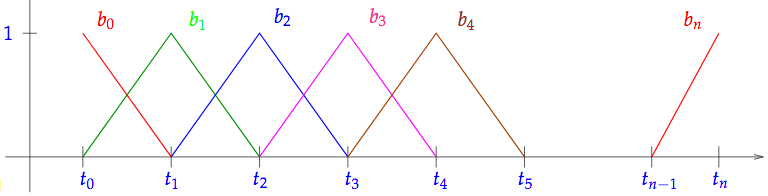
\includegraphics[height=25px, width=\columnwidth,]{5_tent.png}
\end{center}

\Method[Cubic Hermite Interpol.] \\
$\rightarrow$ f $\in C^{1}\left(\left[t_{0}, t_{n}\right]\right)$ \\
Idea: Interpolate each interval as cubic polynomial but edge points have to match, and derivatives on edges have to match. But we have to decide what we want derivates to be at edge:
\begin{itemize}
	\item Linear: (weighted mean of adjacent derivatives) -> No Preservation of monotonicity
	\item Pchip: Since slope must be zero at boundary in some cases -> Loss of linearity
\end{itemize}

\section{Splines}
Instead of fixing the boundary slopes, we add additional continuity constraints. The interpolating function $f$ is then in the Spline Space.\\

\Def[Spline Space] 
$${\scriptstyle
\mathcal{S}_{d, \mathcal{M}}:=\left\{s \in C^{d-1}(I): s_{j}:=s_{\mid\left[t_{j-1}, t_{j}\right]} \in \mathcal{P}_{d} \forall j=1, \ldots, n\right\}}
$$
$\mathcal{S}_{d, \mathcal{M}}$ is the space of piecewise polynomial functions in $C^{d-1}$. One can easily see that $$
\operatorname{dim} \mathcal{S}_{d, \mathcal{M}}=n+d
$$

\Method[Cubic Spline Interpolation] The cubic spline interpolant is a function $s \in \mathcal{S}_{3, \mathcal{M}}$ that complies with the $n+1$ interpolation conditions. Note that we still have 2 degrees of freedom, this leads to the following flavours:
\begin{itemize}
	\item natural: $s^{\prime}\left(t_{0}\right)=0, s^{\prime}\left(t_{n}\right)=0$
	\item periodic: $s^{\prime}\left(t_{0}\right)=s^{\prime}\left(t_{n}\right), s^{\prime\prime}\left(t_{0}\right)=s^{\prime\prime}\left(t_{n}\right)$
	\item complete: $s^{\prime}\left(t_{0}\right)=c_{0}, s^{\prime}\left(t_{n}\right)=c_{n}$
\end{itemize}
The resulting functions is in $C^2$, weakly-local and not strictly shape preserving.

\section{Trigonometric Interpol.}
bla

\section{Least Squares Data Fitting}
\textbf{Goal:} Given $m$ data points $(t_i, y_i)$ and a set of functions $V$, find a continuous function $f\in V$ such that
$$
f \in \underset{\mathbf{g} \in S}{\operatorname{argmin}}\|\textbf{g}(t_i)-y_i\|_{2}^{2}
$$
We focus on \textbf{linear} data fitting, i.o.w. let $V$ be an $n$-dimensional vector space spanned by functions $b_1(t), \dots, b_n(t)$. We look for coefficients 
$$[x_1,\dots,x_n]^T=\underset{\mathbf{z} \in \mathbb{R}^{n}}{\operatorname{argmin}} \sum_{i=1}^{m}\left|\sum_{j=1}^{n}(\mathbf{z})_{j} b_{j}\left(t_{i}\right)-y_{i}\right|^{2}$$

\Theorem[Linear Data Fitting Solution] \\
The solution to the linear least squares fitting problem is the least squares solution of the system
$$
\left[\begin{array}{ccc}
b_{1}\left(t_{1}\right) & \ldots & b_{n}\left(t_{1}\right) \\
\vdots & & \vdots \\
b_{1}\left(t_{m}\right) & \ldots & b_{n}\left(t_{m}\right)
\end{array}\right]
\vx = \left[\begin{array}{c}
y_{1} \\
\vdots \\
y_{m}
\end{array}\right]
$$

\Method[Regularization] We can punish large oscillations by introducing a regularization term:
$$
f \in \underset{g \in V}{\operatorname{argmin}}\left\{\sum_{i=0}^{n}\left|g\left(t_{i}\right)-y_{i}\right|^{2}+\alpha \int_{a}^{b}\left|g^{\prime \prime}(t)\right|^{2} \mathrm{~d} t\right\}
$$

\end{multicols*}
\end{document}
